%   Filename    : chapter_4.tex 
\chapter{Research Methodology}
In this chapter, it outlines a clear and detailed description of the research methods and processes used in the development and evaluation of SeaExchange: A Blockchain Driven App for Tuna Supply Chain Management. The algorithms, systems, theories, framework and models are described in detail in which this chapter establishes the foundation of this study .This chapter also explains the data collection method used ensuring the validity and reliability of the results.In addition, the chapter discusses the considerations and potential limitations of this study. Overall, this will serve as a guide for the readers in understanding the structured process of developing the SeaXChange.

\section{Software Development}
Agile development is a kind of software development that prioritizes flexibility. It is an iterative software development approach that lets a project be broken down into phases and emphasizes continuous improvements. For this study, the researchers opted to use agile development since it involves many stakeholders, it operates in a ever-changing environment. Agile development allows the team to adapt to new requirements.
\section{Research Activities}
For this study, the researchers opted for an interview because it enables in-depth exploration of stakeholder perspectives and experiences. 
The identified fisher and supplier client interface will be tested in the perimeters of Jagnee Fishing Corporation in Tiolas, San Joaquin, Iloilo, Philippines. The identified retailers will be the vendors who sourced their tuna products from Jagnee Fishing Corporation. The identified retailer and consumer testers are situated in the Miagao and San Joaquin areas. 

\subsection{Data Gathering}

\begin{itemize}
	\item \textbf{Primary Data:} 
	\begin{itemize}
		\item Stakeholder(Fishermen and Fishing Corporation, Retailers, and Consumers) interviews to identify the use-case and user requirements, interface usability, and adoption challenges.
		\item Observations of existing tuna supply chain processes in local settings.
	\end{itemize}
	\item \textbf{Secondary Data:} 
	\begin{itemize}
		\item Literature review on blockchain applications in supply chain management and product traceability.
		\item Industry reports and regulatory documents related to tuna fishing and supply chain operations.
	\end{itemize}
\end{itemize}

\subsection{Designing and Developing the System}

\begin{enumerate}
	\item \textbf{Software Development Methodology:} The project follows an Agile methodology to ensure continuous iteration, stakeholder involvement, and flexibility in adapting to feedback.
	\item \textbf{Technology Stack:} 
		\begin{itemize}
			\item Front-end Development: React for creating a secure and user-friendly interface for stakeholders, prioritizing simple and responsive user-interface.
			\item Back-end Development: Node.js for managing back-end processes and API integration. Docker for containerization of the project and Window Subsystem for Linux (Ubuntu as the Linux distribution) for setting up the network.
			\item Blockchain Framework: Go language for developing smart contracts and providing an immutable ledger for transaction data.
		\end{itemize}
	\item \textbf{Blockchain Development Platform:} 
		\begin{itemize}
			\item Hyperledger Fabric for its permissioned nature and scalable architecture.
			\item The open-sourced resources and timely updates of Hyperledger Fabric components is ideal for creating a distributed ledger for tuna supply chain.
		\end{itemize}
\end{enumerate}

\subsection{Implementing Algorithms and Services}
The system for this study is built on top of a Hyperledger Fabric project, it also utilized combinations of algorithms to facilitate the work flow of data or asset as well as ensuring high security with encryption and decryption configuration techniques. 
	\begin{enumerate}
		\item \textbf{Consensus Algorithm} \\The project follows Raft(Leader-based consensus) for handling organizations or nodes. Raft is intended for managing a replicated log in a blockchain network. Raft is a Crash Fault Tolerant (CFT) protocol, is designed to handle non-malicious node failures (e.g., hardware crashes, network issues) In Raft, one node is elected as the leader, and it coordinates the ordering of transactions (Xu et al, 2022) \nocite{method-1}. The leader replicates log entries (transactions) to follower nodes, ensuring consistency across the network. 
		
		\item \textbf{Cryptographic Algorithm} \\The project employs several cryptographic algorithms to ensure security and privacy. These cryptographic data serves as digital signatures and identity verification for the project. ECDSA (Elliptic Curve Digital Signature Algorithm) is used for generating digital signatures while X.509 certificates are intended for identity management and authentication of participants (Anitha \& Sankarasubramanian, n.d.) \nocite{method-2}. For the encryption, AES (Advanced Encryption Standard) is used for encrypting data at rest and in transit. TLS (Transport Layer Security) secures communication between network nodes. SHA-256 (Secure Hash Algorithm-256) ensures data integrity by generating unique hashes for blocks and transactions.
		
		\item \textbf{Membership Service} \\The implementation of the Membership Service Provider (MSP) requirement involves a set of folders added to the network configuration. These folders define an organization both internally, by specifying its administrators, and externally, by enabling other organizations to verify the authority of entities attempting specific actions. While Certificate Authorities (CAs) are responsible for generating the certificates that represent identities, the MSP includes a list of permitted identities. The MSP specifies which Root CAs and Intermediate CAs are authorized to define members of a trust domain. This is achieved by either listing the identities of their members or identifying the CAs allowed to issue valid identities for those members.
		
		\item \textbf{Ordering Service} \\ The ordering service in this study plays a crucial role in maintaining the integrity and functionality of the blockchain network. Its primary responsibilities include ensuring that transactions are processed in the correct sequence (transaction ordering), grouping transactions into blocks based on configurable parameters like size or timeout (block creation), and distributing these ordered blocks to peers for validation and commitment (block distribution) (Nassar et al, 2024)\nocite{method-3}. Additionally, the ordering service provides fault tolerance to ensure the network remains operational even in the presence of node failures through Raft.
		
		\item \textbf{Endorsement Policy} \\Fabric employs endorsement policies to specify which peers must validate a transaction before it's committed. The algorithm involves multi-signature schemes where a transaction is valid if it receives endorsements from the required peers as per the policy.
		
		\item \textbf{Chaincode (Smart Contract)} \\The handling and flow of business logic agreed to by members of the tuna supply chain in the blockchain network is executed by a chaincode or smart contract. The chaincode of the app is written in Go language. Docker container is used for enabling the chaincode to securely run along with the overall hyperledger fabric configurations. Chaincode initializes and manages ledger state through transactions submitted by applications (Hyperledger Fabric Documentation, 2024) \nocite{method-4}. The chaincode follows the object-oriented paradigm for creating classes and objects necessary for the tuna supply chain.
		
		
	\end{enumerate}

\subsection{Modeling the System Architecture}
The system architecture of the project consists of many nodes that communicate with each other. The chaincode enables the system to run algorithms, particularly, holding state and ledger data, and executes transactions such as asset transfer in the tuna supply chain. 

	\begin{itemize}
		\item \textbf{Blockchain Architecture}
		\\The project involves peer, ordering services, ledger, and client application to perform various transaction such as tracing the origin and the stop points of a tuna asset. Peers are nodes in the blockchain network that maintain a copy of the distributed ledger and execute chaincode (smart contracts). The ordering service is the central component of the blockchain for ordering transactions and creating blocks to distribute to peers through consensus mechanism. The ledger is the immutable record of all transaction in the tuna supply chain network, stored across all peers. The client application is the interface through which users or tuna supply chain participants interact with the blockchain network.
		
		\begin{figure}[H]
			\centering
			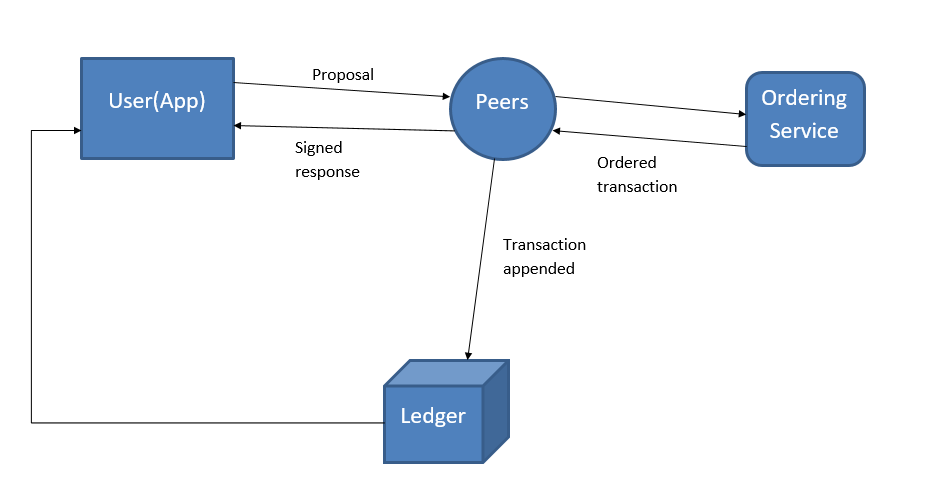
\includegraphics[width=0.8\textwidth]{SeaXChange_model.png}
			\caption{Blockchain Architecture of SeaXChange}
			\label{fig:blockchain_model}
		\end{figure}
		
		
		
		\item \textbf{Use Case}
		\\The use case shows the outline on how the user will interact with the SeaExchange App. It will follow the major stages or participants in the tuna supply chain. 
		\begin{enumerate}
			\item \textbf{Fishing Vessel}
			\\- Encodes batch I.D. of fish.
			\\- Encodes the date when the fish was captured.
			\\- Encodes the location where the fish was captured.
			\\- Encodes the fishing method used.
			\\- Query the origin and exchange of the tuna asset.
			
			\item \textbf{Supplier}
			\\- Encodes when the product was transferred from fishing vessel to supplier.
			\\- Query the origin and exchange of the tuna asset.
			\\- Generate supplier's location during retrieval of tuna asset.
			
			\item \textbf{Retailer}
			\\- Encodes when the product was retrieved from the supplier.
			\\- Query the origin and exchange of the tuna asset.
			\\- Generate retailer's location during retrieval of tuna asset.
			
			\item \textbf{Consumer}
			\\- Retrieve data from retailer.
			\\- Query the origin and exchange of the tuna asset.
			\\- Generate user's address during retrieval of tuna asset.
		
			\begin{figure}[h]  
				\centering
				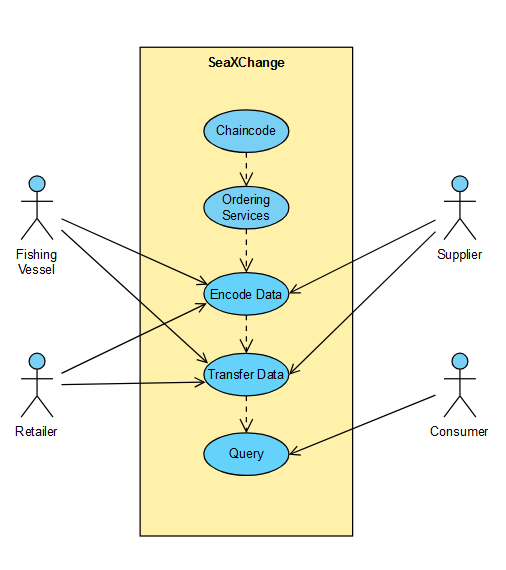
\includegraphics[width=0.8\textwidth]{UseCase.png}
				\caption{Use case diagram for SeaXchange.}
				\label{fig:usecase}  
			\end{figure}
			
		\end{enumerate}
	\end{itemize}

\clearpage
\newpage
\section{Calendar of Activities}
%
%  the following commands will be used for filling up the bullets in the Gantt chart
%
\newcommand{\weekone}{\textbullet}
\newcommand{\weektwo}{\textbullet \textbullet}
\newcommand{\weekthree}{\textbullet \textbullet \textbullet}
\newcommand{\weekfour}{\textbullet \textbullet \textbullet \textbullet}

%
%  alternative to bullet is a star 
%

\begin{table}[H]
	\centering
	\caption{Timetable of Activities} \vspace{0.25em}
	\resizebox{\textwidth}{!}{%
		\begin{tabular}{|>{\centering\arraybackslash}p{1.5in}|c|c|c|c|c|c|c|c|c|c|c|c|}
			\hline
			Activities (2024) & Aug & Sep & Oct & Nov & Dec & Jan & Feb & Mar & Apr & May & Jun \\ \hline
			Brainstorming and Selection of Topic   & \weekone & \weektwo &  &  &  &  &  &  &  &  &  \\ \hline
			Review of Related Literature & \weekthree & \weekfour &  &  &  &  &  &  &  &  &  \\ \hline
			Interview Potential Stakeholders      &  & \weektwo  & \weekfour & \weekone &  &  &  &  &  &  &  \\ \hline
			Proposal Document Creation in LaTex     &   &  &  & \weekfour & \weekfour &  &  &  &  &  &  \\ \hline
			Mockups and Prototype      &   &  &  & \weektwo & \weekfour &  &  &  &  &  &  \\ \hline
			Proposal Presentation &   &  &  &  & \weekone &  &  &  &  &  &  \\ \hline
			Development and Testing of Software &  &  &  &  &  & \weekfour & \weekfour & \weekfour & \weekfour & \weekfour & \weekone \\ \hline
			Deployment of Software &  &  &  &  &  &  &  &  &  &  & \weekone \\ \hline
			Results and Feedback  &  &  &  &  &  &  &  &  &  &  & \weekone \\ \hline
		\end{tabular}%
	}
	\label{tab:timetableactivities}
\end{table}

